\section{Righe Spettrali}\label{sec:righe-spettrali}

\subsection{Opacità per l'atmosfera stellare}\label{sec:opacità-atmosfera}
Un parametro importante per la determinazione di un modello per l'atmosfera stellare è l'opacità, già discussa nel par.~\ref{sec:opacità}. Ripassiamo i concetti principali. I processi che determinano l'opacità di una struttura sono:
\begin{description}
    \item[BB] discusso nel par.~\ref{sec:bound-bound}. Avviene a una determinata lunghezza d'onda, secondo l'eq.~\eqref{eq:lunghezza-BB}. È responsabile delle \emph{righe di assorbimento}, poiché determinano la mancanza di flusso a una determinata lunghezza d'onda.
    \item[BF] discusso nel par.~\ref{sec:bound-free}. Contribuisce all'opacità del \emph{continuo}.
    \item[FF] discusso nel par.~\ref{sec:free-free}. Contribuisce all'opacità del \emph{continuo}.
    \item[E] discusso nel par.~\ref{sec:electron-scattering}. Contribuisce all'opacità del \emph{continuo}.
\end{description}
In particolare, nelle atmosfere le temperature sono sufficientemente basse affinché i fotoni possano essere poco energetici e possano eccitare gli elettroni degli atomi, lasciandoli in stati legati. Dunque il fenomeno del BB, che negli interni stellari trascuravamo a causa delle elevate temperatura, sarà determinante nelle atmosfere. La velocità di variazione dell'opacità con la lunghezza d'onda determina come l'opacità stessa si manifesta, ovvero in forma di righe di assorbimento o nel continuo. Vediamo degli esempi.

\paragraph{Esempio--Serie di Balmer}
\paragraph{Esempio--Balmer Jump}

\subsection{Continuo spettrale e righe spettrali di assorbimento}

\subsection{Classificazione spettrale delle stelle}
Come visto nel par.~\ref{sec:opacità-atmosfera}, l'\emph{atmosfera} stellare è dove si formano il \emph{continuo spettrale} e le \emph{righe spettrali di assorbimento}. Le righe di assorbimento, in particolare, sono degli osservabili fondamentali perché è dalla loro intensità che possiamo misurare l'\emph{abbondanza} dei diversi elementi chimici. Si faccia attenzione al seguente fatto: la presenza o meno di una data riga spettrale \emph{non} dipende dalla presenza o meno di quel dato elemento, ma è fortemente modulata dalla \emph{temperatura}. Vediamo di chiarire il fatto.

Ovviamente, se un elemento non è presente nella struttura stellare, lo spettro non potrà mostrare le sue righe. Tuttavia, l'assenza di righe di un dato elemento \emph{non necessariamente} significa che quel dato elemento è assente: potrebbe esserci, ma la \emph{temperatura} non è tale da far manifestare le sue righe. Infatti, le righe di assorbimento sono dovute a fenomeni di eccitazioni o ionizzazioni della materia e, come noto,  il numero di stati eccitati o ionizzati dipende primariamente dalla temperatura. Se, ad esempio, la temperatura non è sufficientemente alta da far sì che tutti gli atomi di un dato elemento siano ionizzati, non potrò mai vedere la riga di assorbimento di tale elemento, anche se è presente.

In definitiva, è la temperatura che modula in manifestarsi delle righe spettrali, ovvero è la \emph{temperatura} che determina il \emph{tipo spettrale} delle stelle. Dunque, le stelle sono classificate in base al loro tipo spettrale, ovvero in base alla presenza e all'intensità delle varie righe spettrali, il quale, a sua volta, riflette il valore della temperatura atmosferica della stella.

\begin{figure}
    \centering
    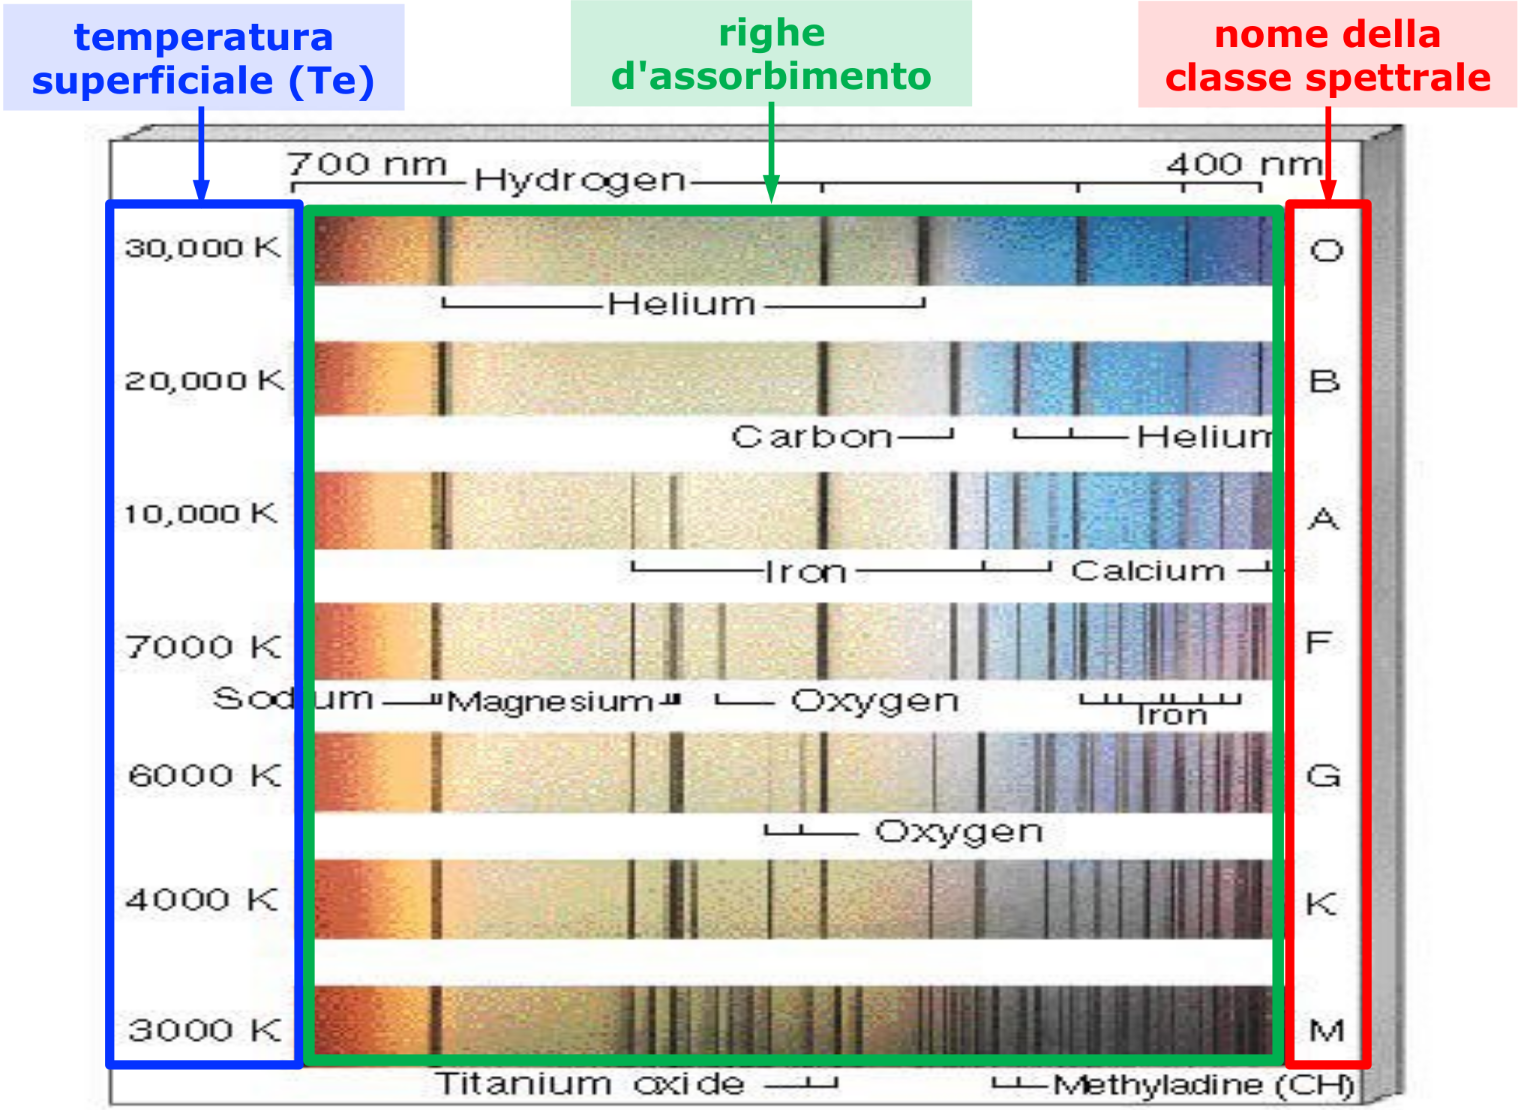
\includegraphics[width=0.7\textwidth]{immagini/classificazione-spettrale-stelle.png}
    \caption{Classi spettrali principali.}
    \label{fig:classificazione-spettrale-stelle}
\end{figure}

Nella fig.~\ref{fig:classificazione-spettrale-stelle} sono rappresentate le principali \emph{classi spettrali}, elencate anche di seguito:
\begin{description}
    \item[O]
    \item[B]
    \item[A]
    \item[F]
    \item[G]
    \item[K]
    \item[M]
\end{description}
Si può ricordare tale lista con la seguente frase: \emph{"O,B,A, Fine Girl Kiss Me"}.

\subsection{Equazione di Boltzmann}
\subsection{Equazione di Saha}
\subsection{Velocità radiale}
\subsection{Abbondanze chimiche}
\subsubsection{Larghezza equivalente}
\subsection{DA SCRIVERE Altre cose e Recap}